\documentclass[12pt]{article}
\usepackage{geometry}                % See geometry.pdf to learn the layout options. There are lots.
\geometry{letterpaper}                   % ... or a4paper or a5paper or ... 
%\geometry{landscape}                % Activate for for rotated page geometry
\usepackage[parfill]{parskip}    % Activate to begin paragraphs with an empty line rather than an indent
\usepackage{daves,fancyhdr,natbib,graphicx,dcolumn,amsmath,lastpage,url}
\usepackage{amsmath,amssymb,epstopdf,longtable}
\usepackage[final]{pdfpages}
\DeclareGraphicsRule{.tif}{png}{.png}{`convert #1 `dirname #1`/`basename #1 .tif`.png}
\pagestyle{fancy}
\lhead{CE 3354 -- Engineering Hydrology}
\rhead{FALL 2024}
\lfoot{PR11}
\cfoot{}
\rfoot{Page \thepage\ of \pageref{LastPage}}
\renewcommand\headrulewidth{0pt}



\begin{document}
\begin{center}
{\textbf{{ CE 3354 Engineering Hydrology} \\ {Team Project 1}}}
\end{center}

\section*{\small{Problem Statement}}
Figure \ref{fig:Concho3} is a map of a portion of Concho County, Texas.  In the Southeast corner of the map is Eden, Texas.  A US highway runs nearly East-West through Eden, and another US highway runs North-South.
%%%%%%%%%%%%%%%%%%%%%%%%%%%%%%%%%%%%%%%%%%%%%%%%
\begin{figure}[h!] %  figure placement: here, top, bottom, or page
   \centering
   \includegraphics[width=6in]{Concho3.png} 
   \caption{Harden Branch Creek near Eden, Texas}
   \label{fig:Concho3}
\end{figure}
%%%%%%%%%%%%%%%%%%%%%%%%%%%%%%%%%%%%%%%%%%%%%%%%%
To the East of town, a culvert system is to be replaced by a bridge.   The removal of the culvert is anticipated to reduce temporary storage on the upstream side of the East-West highway and convey water to another crossing South of town.  

The overall task is to assess the impact of the increased conveyance conferred by the bridge (in place of the existing 3-barrel 8X8 box culvert system) on the downstream portion of the stream between the bridge and the next downstream crossing.

Questions to be addressed are:
\begin{enumerate}
\item Does the downstream structure also need change to maintain the pre-development (current) conditions?
\item If the downstream is unchanged, is there substantial change in inundation potential for the structures on the Southwest corner of Eden (see the map).
\item The area between the two roads is currently a golf course – a reasonably compatible land use for an area that from time to time is inundated. A developer desires to build executive homes adjacent to the golf course, where should those homes be located? (i.e. estimate a regulatory base-flood-elevation)
\end{enumerate}

Perform and document a study in an engineering report, with appendices as necessary that contain the underlying data or assumptions employed. The analysis anticipates that HEC-HMS will be used for hydrology up to the culvert system (or bridge) on US 87, and to the next structure on US 83

Report Requirements:

The engineering project report should consist of the following (minimal) contents.
\begin{enumerate}
\item Letter of Transmittal
\item Executive Summary
\item Introduction (background information, methods and procedures, etc.)
\item Hydrologic Analyses of Existing System including:
\begin{itemize}
\item Watershed Delineation: There are two “points” of interest. The crossing at US 87 and the crossing at US 83, these are the red circles on Figure \ref{fig:Concho3}. The two upstream reservoirs themselves become points of interest as they have their own sub-basins that are part of the larger system. A reasonable delineation will likely identify four sub-basins: two for each reservoir, one that drains directly to the culvert/bridge on US 87, and one for the area between US 87 and US 83.
\item Annual Recurrence Interval: Select from the Hydraulic Design Manual of appropriate risk levels for the crossings. Bear in mind, we would like the crossings to convey the “design risk” without overtopping the roadway. The 1\% chance is also to be considered, in this study to examine the impact on the golf course area. In this project, the 1\% chance event, if necessary can overtop the system, but the design risk should pass both structures. The relevant section of the Hydraulic Design Manual is attached.
\item Design Storm: Determine an appropriate design storm based on the ARI above and the watershed area. Include explanation of how storm duration was selected.
\item Loss (Runoff Generation) Model: Determine an appropriate loss model based on watershed size and land cover. Document how you determined parameters of your selected loss model.
\item Transformation Model: Using the SCS unit hydrograph model, determine appropriate parameterization for each of the sub-basins. Document how you determined the model parameters.
\item Routing Model: Explain how reservoir flows are routed to the structure(s). For example there will be routing from the two reservoirs to the US 87 culvert, then routing from US 87 to US 83.
\item Water Surface Elevations: The culvert system on US 87 is a 3- barrel 6 X 6 box culvert system. The culvert system on US 83 is a 5-barrel 6-foot diameter circular culvert system. Document how you estimate the water surface elevations at the culvert systems under different design conditions. If you choose a routing model that can report depths, state so in the report.
\end{itemize}
\item System Design Modifications
\begin{itemize}
    \item Compare the pre-development conditions with the post development conditions. You can assume the bridge behaves as if the channel is unobstructed – you can estimate width from the map.
    \item Repeat the analysis (run a model with modified routing) to determine the impact at the US 83 crossing and the possible development described in the problem statement.
\end{itemize}
\item Summary and Recommendations
\item References
\item Appendix (sample calculations, data, etc.)
\end{enumerate}

Additional Guidance:

The two reservoirs are SCS reservoirs designed to capture and release water over 7 days. That is, once full but not over the spillway, the reservoir should drain in about a week. Use that information to approximate an appropriate release mechanism in the simulation model(s). (Probably an orifice and weir arrangement, but read the user manual for other possibilities)

You will have to construct some kind of storage curves for the reservoirs and may have to use algebra and curve fitting to complete such curves. Pursuant to those curves, there will be some kind of stage-discharge relationship. You may assume that the spillways crest about 4 feet below the dam crests and the spillways are about 50 feet wide.

\clearpage

Figure \ref{fig:aerial}, is an aerial image of the area for some additional geomorphic context.

%%%%%%%%%%%%%%%%%%%%%%%%%%%%%%%%%%%%%%%%%%%%%%%%
\begin{figure}[h!] %  figure placement: here, top, bottom, or page
   \centering
   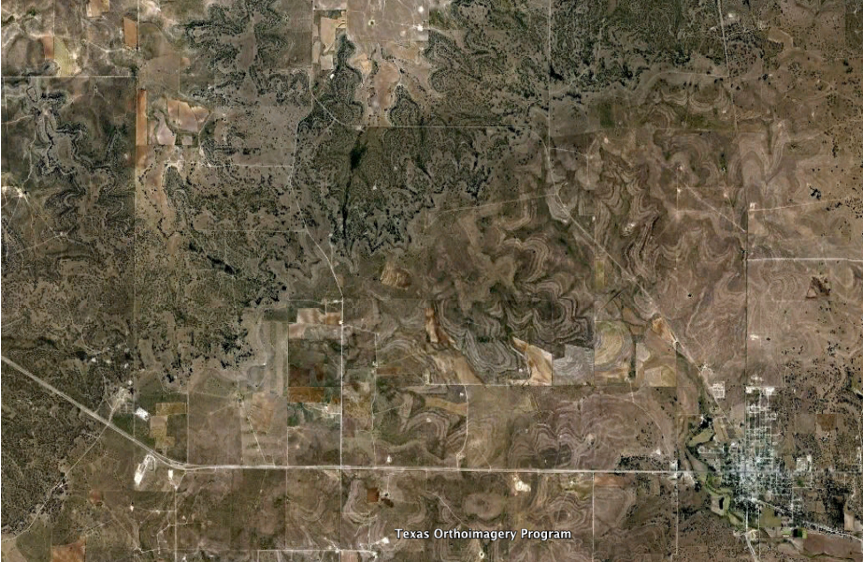
\includegraphics[width=6in]{aerial.png} 
   \caption{Harden Branch Creek near Eden, Texas}
   \label{fig:aerial}
\end{figure}
%%%%%%%%%%%%%%%%%%%%%%%%%%%%%%%%%%%%%%%%%%%%%%%%%

\clearpage

Figure \ref{fig:background}, is a map  of the area for showing the two points of interest without any annotations.

%%%%%%%%%%%%%%%%%%%%%%%%%%%%%%%%%%%%%%%%%%%%%%%%
\begin{figure}[h!] %  figure placement: here, top, bottom, or page
   \centering
   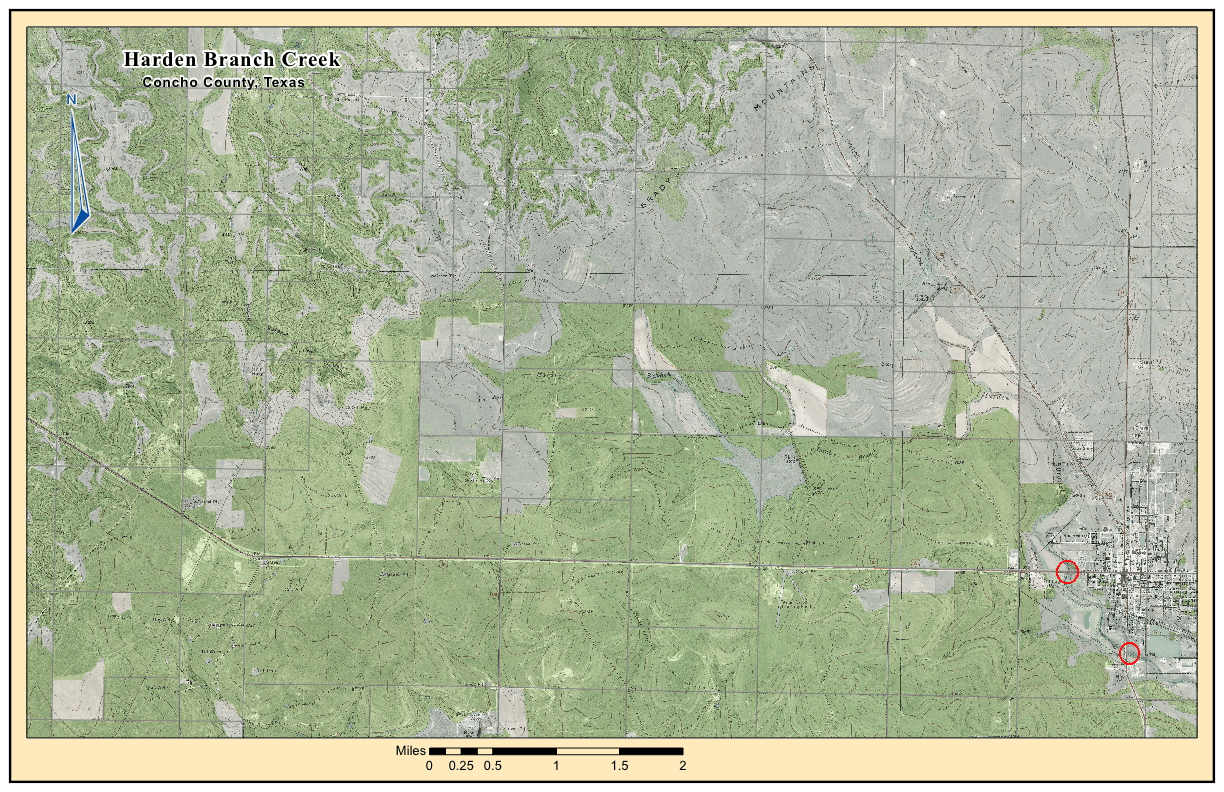
\includegraphics[width=6.5in]{Concho-Background-POI.png} 
   \caption{Harden Branch Creek near Eden, Texas}
   \label{fig:background}
\end{figure}
%%%%%%%%%%%%%%%%%%%%%%%%%%%%%%%%%%%%%%%%%%%%%%%%%

\clearpage

Figure \ref{fig:hmslayout}, is a map of the study area broken into suggested sub-basins for hydrologic/hydraulic analysis.  The software in the image is a digitizer that predates easy access to GIS, but helps accomplish the same tasks.

%%%%%%%%%%%%%%%%%%%%%%%%%%%%%%%%%%%%%%%%%%%%%%%%
\begin{figure}[h!] %  figure placement: here, top, bottom, or page
   \centering
   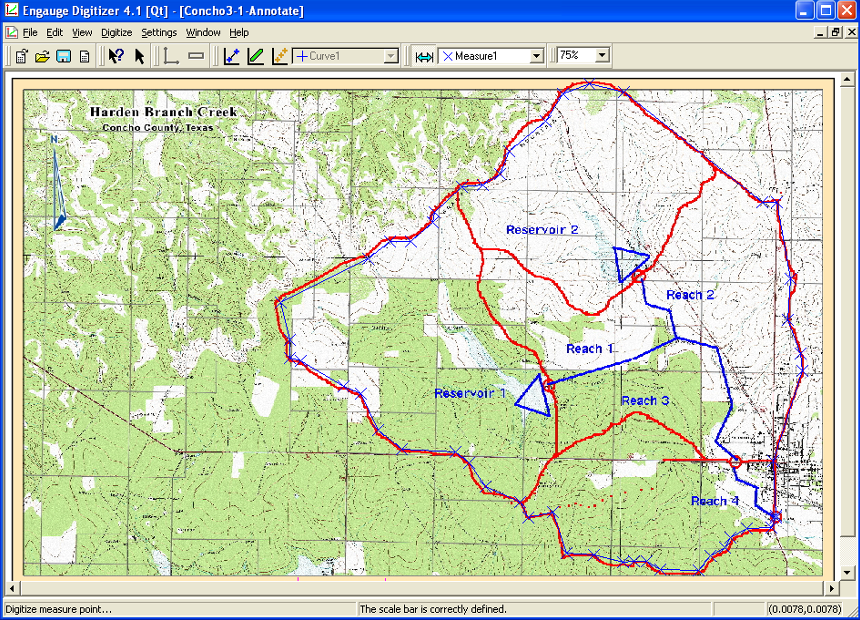
\includegraphics[width=6in]{layout.png} 
   \caption{Harden Branch Creek HEC-HMS Layout near Eden, Texas}
   \label{fig:hmslayout}
\end{figure}
%%%%%%%%%%%%%%%%%%%%%%%%%%%%%%%%%%%%%%%%%%%%%%%%%

\clearpage

Figure \ref{fig:effortsheet}, is a suggested effort sheet to use to manage your team's project.  The sheet should be updated weekly (and the weekly sheets included in the report appendix)
%%%%%%%%%%%%%%%%%%%%%%%%%%%%%%%%%%%%%%%%%%%%%%%%
\begin{figure}[h!] %  figure placement: here, top, bottom, or page
   \centering
   
\includegraphics[height=7in]{effortsheet.png} 
   \caption{Project Management Effort Sheet}
   \label{fig:effortsheet}
\end{figure}
%%%%%%%%%%%%%%%%%%%%%%%%%%%%%%%%%%%%%%%%%%%%%%%%%

\clearpage

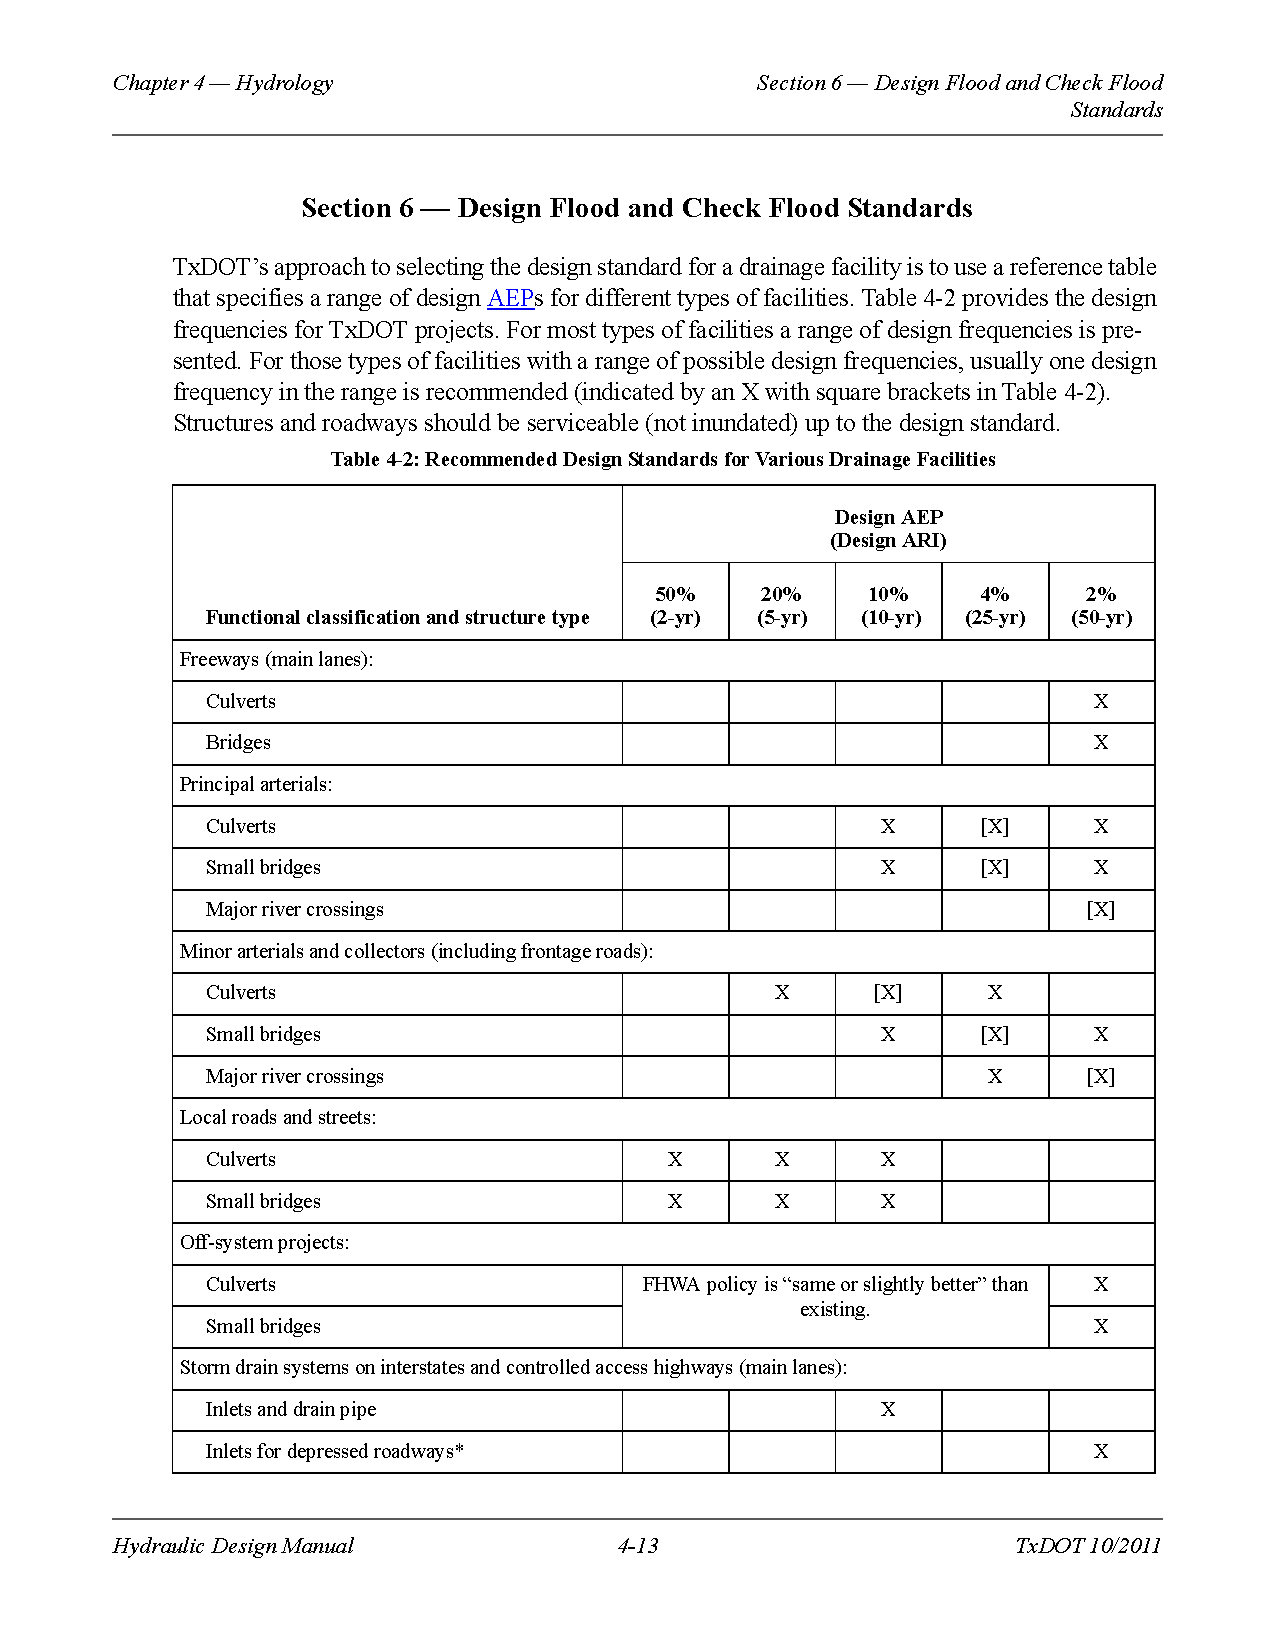
\includepdf[pages={-}]{./Pages_from_hyd.pdf}

\end{document}  

%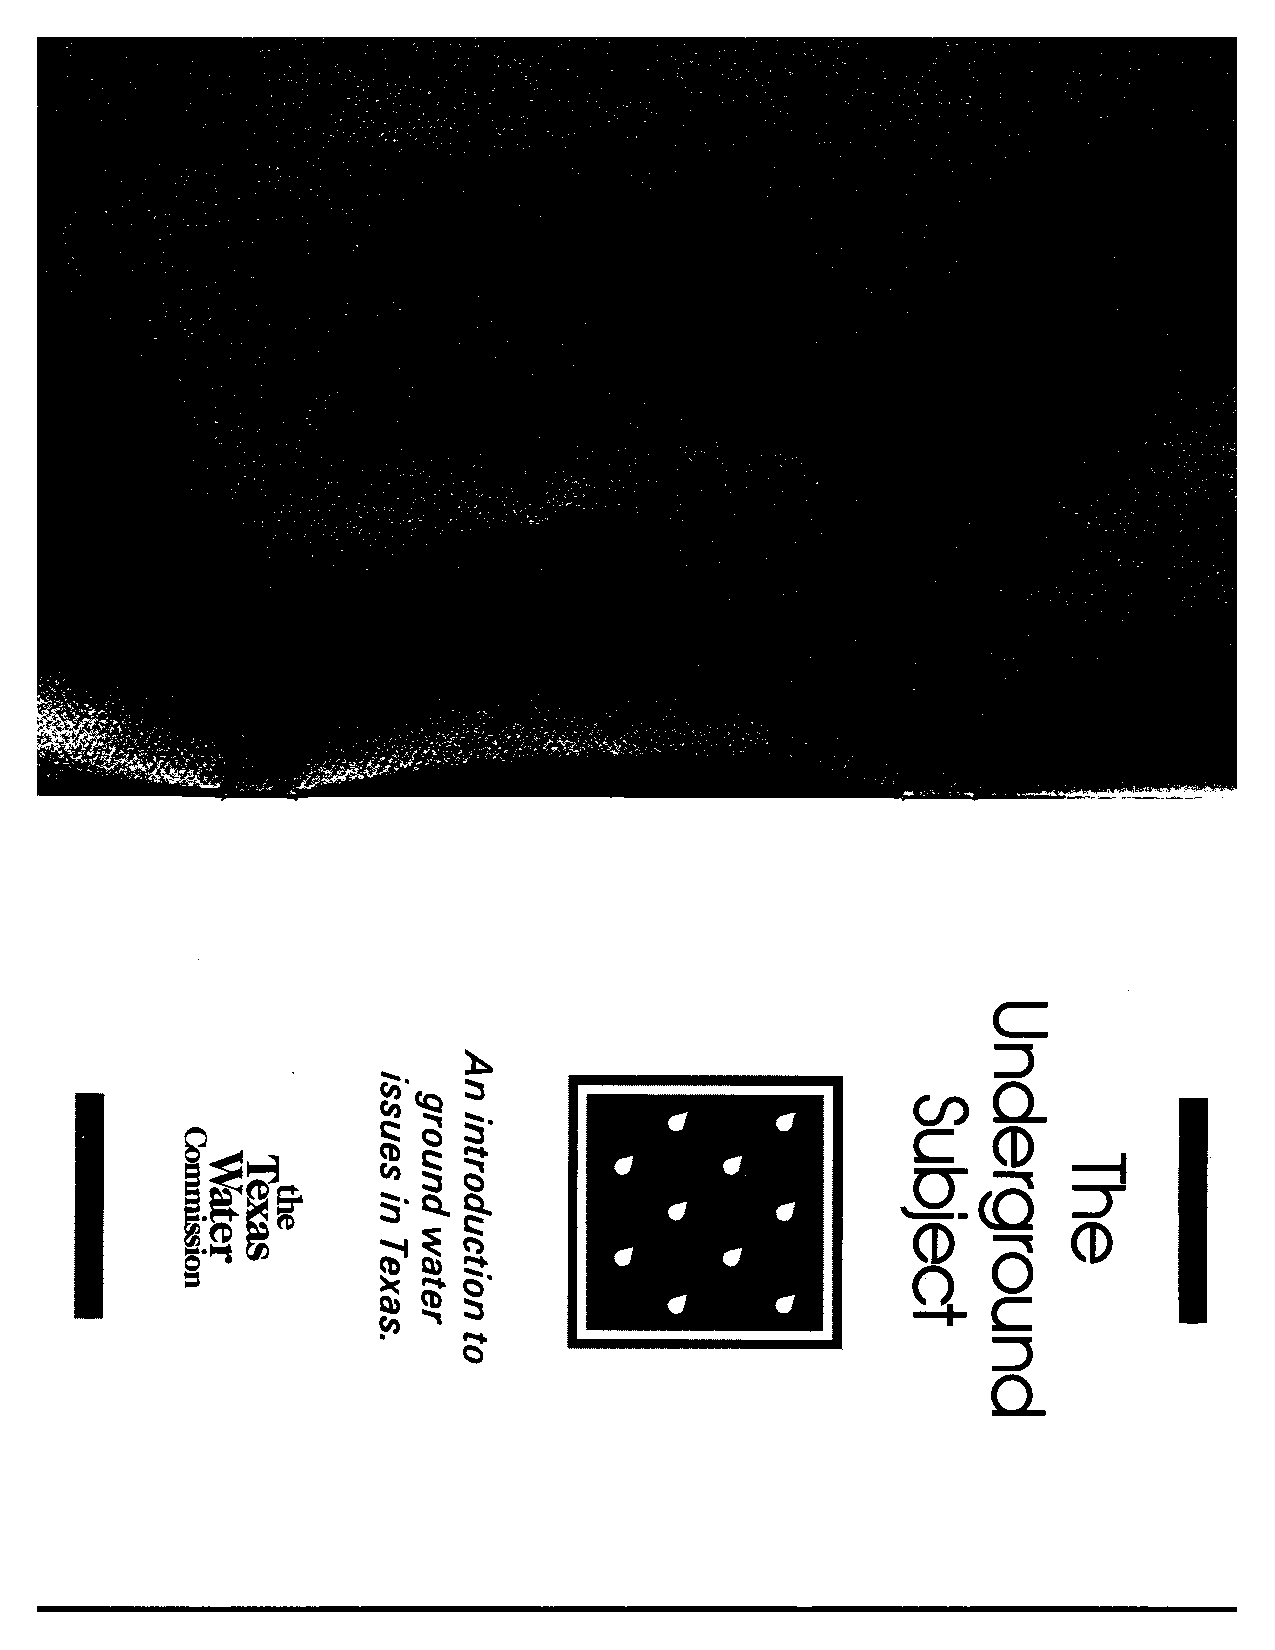
\includepdf[pages={-}]{./TWC_8905.pdf}
 
\item Figure \ref{fig:farmland} is a schematic of a 600-hectare farm; the land receives annual rainfall of 2500 mm.  There is a river flowing through the farm land with inflow rate of 5 m$^3$/s and outflow rate of 4m$^3$/s.  The annual water storage in the farm land increases by 2.5$\times$10$^6$m$^3$.  Using the water budget concept, estimate the annual evaporation amount in millimeters.\footnote{1 hectare = 10,000 m$^2$}

\begin{figure}[h!] %  figure placement: here, top, bottom, or page
   \centering
   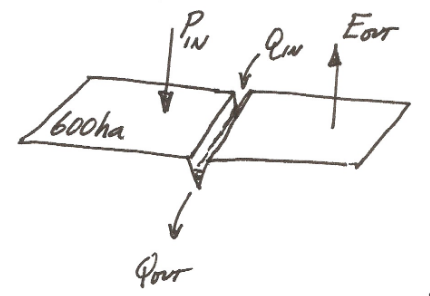
\includegraphics[width=4in]{farmland.png} 
   \caption{Schematic of Farmland}
   \label{fig:farmland}
\end{figure}

\item A reservoir has a surface area of 690 acres.  Figure \ref{fig:reservoir} shows the monthly inflow of surface water, outflows as releases from the reservoir via the spillway, direct precipitation into the reservoir, and evaporation from the reservoir.  The reservoir water surface elevation was 701.0 feet on January 1.  Determine the reservoir water surface elevation at the end of each month (i.e. complete the table)

\begin{figure}[h!] %  figure placement: here, top, bottom, or page
   \centering
   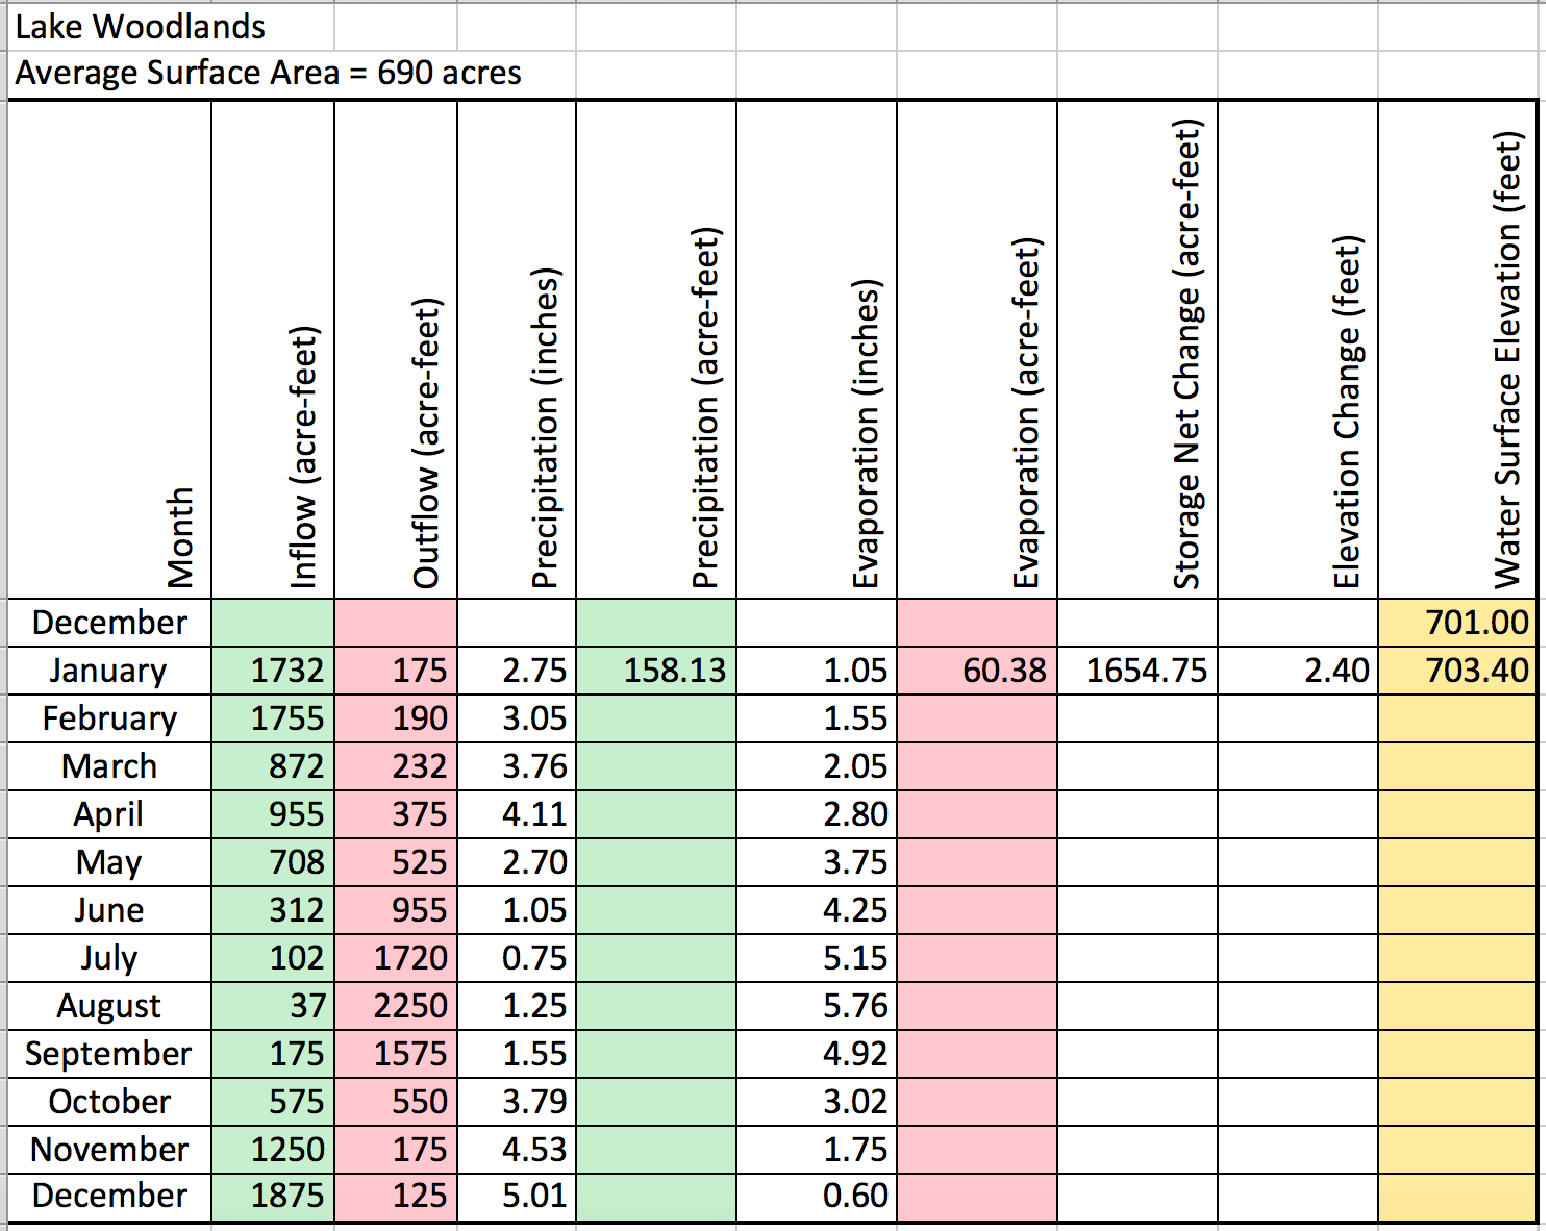
\includegraphics[width=6in]{Reservior.pdf} 
   \caption{Tabular Water Budget Values}
   \label{fig:reservoir}
\end{figure}